\chapter{Elaboració d'una App per Practicar la Memorització}
\label{cha:python}

En saber tots aquests conceptes vaig decidir que hauria de portar aquesta eficiència a l'hora
de resoldre, a l'aprenentatge. És a dir, que a la vegada que per resoldre el cub a cegues es
busca l'eficiència en cada pas, però a l'hora d'aprendre tota aquesta llista de conceptes és un
procés molt lent. I és per això que per posar en pràctica el procés de memorització és a dir traduir les lletres a les paraules per visualitzar imatges, el que vaig fer és una aplicació que et
generi lletres, després te les amagui i tu hagis de posar les lletres que has memoritzat.
\\\\Aquesta app està realitzada amb el llenguatge de programació Python, i amb la biblioteca tkinter per crear interfície gràfica\footnote{Una interfície gràfica és el que veus dins d'una aplicació, (els botons, menús\dots)}.
\\\\L'app consta de diferents labels\footnote{És un text que l'usuari no pot alterar.}, botons i textboxes\footnote{És una "caixa" on l'usuari pot alterar el text.}, que es mostren es deixen de mostrar segons la funció que es doni i cada una d'aquestes funcions és escollida mitjançant els botons. Durant aquesta explicació del codi cal tenir en compte que les frases de color verd escrites després d'un asterisc són comentaris i no afecten al codi.

\vspace{0.5cm}

Per començar, importem els paquets\footnote{Un paquet és una col·lecció de fitxers i directoris necessaris per a una finalitat de programari} de tkinter i random, que el random es fa servir per generar les lletres aleatòriament. I després de tkinter importem els messageboxes.

\begin{lstlisting}[language=Python, style=colorEX, caption=Importació de paquets]
import tkinter as tk
import random
from tkinter import messagebox
\end{lstlisting}

Després inicio una classe on estarà tot el contingut i de l'app. Just a l'inici d'aquesta classe
especifico el títol de la finestra on es mostra l'app a més a més de les dimensions que tindrà i
el logo que es mostrarà.

\begin{lstlisting}[language=Python, style=colorEX, caption=Inici de la classe i especificació de la finestra]
class MemorizeApp:    
    def __init__(self, root):
        self.root = root
        self.root.title("Memo App by Pol Sances")
        self.root.geometry("500x500")
        self.root.iconbitmap("Brain.ico")
\end{lstlisting}

Després inicio una classe on estarà tot el contingut i de l'app. Just a l'inici d'aquesta classe
especifico el títol de la finestra on es mostra l'app a més a més de les dimensions que tindrà i
el logo que es mostrarà. Just a sota del codi anterior declaro tots els objectes que estaran presents a l'app, labels que
diuen el temps, textbox en la qual l'usuari omple amb un número i botons d'inici i tornar a iniciar
el procediment. Com a referència els objectes comencen amb un self. I la seva continuació és
el nom d'objecte que és. 

\begin{lstlisting}[language=Python, style=colorEX, caption=Declaració d'objectes necessaris pel funcionament de l'App]
        self.letters = self.generate_letters()

        self.label = tk.Label(self.root, text="", font=("Arial", 24))
        self.label.pack(pady=20)

        self.time_entry = tk.Entry(self.root, font=("Arial", 14))
        self.time_entry.insert(0, "Write time in seconds")
        self.time_entry.pack(pady=10)

        self.start_button = tk.Button(self.root, text="Start", command=self.start_memorize)
        self.start_button.pack(pady=5)

        self.answer_entry = tk.Entry(self.root, font=("Arial", 14))
        self.answer_entry.pack(pady=10)

        self.submit_button = tk.Button(self.root, text="Submit", command=self.check_answers)
        self.submit_button.pack(pady=5)

        self.reset_button = tk.Button(self.root, text="Reset", command=self.reset)
        self.reset_button.pack(pady=5)

        self.answer_entry.config(state="disabled")
        self.submit_button.config(state="disabled")
        self.reset_button.config(state="disabled")

        self.name = tk.Label(self.root, text="Made by Pol Sances Guirao", font=("Arial", 8))
        self.name.pack(pady=20)
\end{lstlisting}

Després començo a escriure les funcions, en aquest cas començo amb la funció de generar les lletres gràcies al paquet random. Les funcions a Python comencen amb el def i el nom de la funció, aquesta funció inicia una llista on s'escriuran les lletres generades. A sota on posa for i in range[20], significa que està creant un bucle 20 vegades on es genera una lletra i s'escriu a la llista.

\begin{lstlisting}[language=Python, style=colorEX, caption=Funció per generar lletres]
    def generate_letters(self):
        letters = []
        for _ in range(20):
            letter = chr(random.randint(65, 90))
            letters.append(letter)
        return letters
\end{lstlisting}

Les següents funcions són les de començar a memoritzar, aquestes funcions són les que s'atribueixen al botó d'inici de la memorització. El que fan és desactivar el botó start un cop clicat i
afegir la llista de lletres dins del label perquè l'usuari pugui començar a memoritzar. Abans d'això la funció ha agafat el temps que havia introduït l'usuari i el converteix a mil·lisegons perquè
el programa mostri les lletres la quantitat de temps desitjada a més a més d'amagar les lletres
a l'usuari.

\begin{lstlisting}[language=Python, style=colorEX, caption=Funcions pel botó d'inici]
    def start_memorize(self):
        self.start_button.config(state="disabled")
        self.label.config(text="".join(self.letters))
        time_delay = int(self.time_entry.get()) * 1000  # Convert user seconds to milliseconds
        self.root.after(time_delay, self.show_entry)
        self.time_entry.pack_forget()

    def show_entry(self):
        self.label.config(text="")
        self.answer_entry.config(state="normal")
        self.submit_button.config(state="normal")
        self.reset_button.config(state="normal")
        self.answer_entry.focus_set()
\end{lstlisting}

La següent funció és la de comprovar la resposta que has introduït, quan fas clic en el botó
d'enviar la resposta, el que fa és dir-te si la resposta és correcta o incorrecta. I activar el botó
de reset per poder tornar a començar.

\begin{lstlisting}[language=Python, style=colorEX, caption=Funció per comprovar la resposta]
    def check_answers(self):
        user_answers = self.answer_entry.get().upper()
        correct_answers = "".join(self.letters)

        if user_answers == correct_answers:
            messagebox.showinfo("Result", "Correct answers!")
        else:
            messagebox.showinfo("Result", "Incorrect answers. Try again.")

    self.reset()
\end{lstlisting}

L'última funció és la de tornar a començar, la qual et torna a generar les lletres i torna a
començar el compte enrere, de manera resumida, torna a l'estat on li havies fet clic en el botó
d'inici.   

\begin{lstlisting}[language=Python, style=colorEX, caption=Funció per tornar a començar]
    def check_answers(self):
        user_answers = self.answer_entry.get().upper()
        correct_answers = "".join(self.letters)

        if user_answers == correct_answers:
            messagebox.showinfo("Result", "Correct answers!")
        else:
            messagebox.showinfo("Result", "Incorrect answers. Try again.")

        self.reset()
\end{lstlisting}

Finalment, tenim la part més important del codi que és el que crea la finestra principal i s'executa el bucle principal (mainloop) per mantenir l'aplicació en funcionament.

\begin{lstlisting}[language=Python, style=colorEX, caption=Bucle per mantenir l'aplicació en funcionament]
if __name__ == "__main__":
    root = tk.Tk()
    app = MemorizeApp(root)
    root.mainloop()
\end{lstlisting}

El codi complet es pot veure a l'annex 1 i el resultat del codi executat en les diferents fases es pot veure a les figures \ref{fig:fase-incial}, \ref{fig:fase-memo}, \ref{fig:fase-resp}. \cite{Freecodecamp} \cite{Tkinter} \cite{LogoCervell} \cite{RecursosPython}

\begin{figure}[h!]
    \centering
    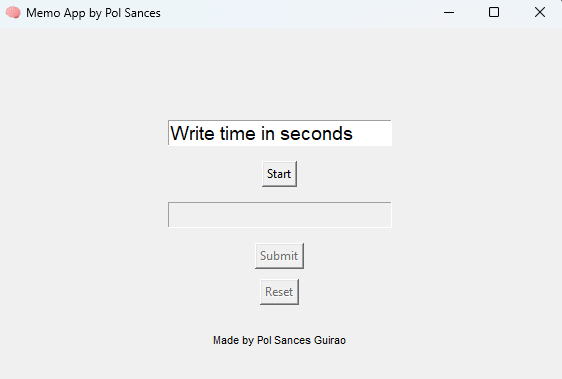
\includegraphics[width=8cm]{img/figures/app-fase1.png}
    \caption{Fase Incial}
    \label{fig:fase-incial}
\end{figure}

\begin{figure}[h!]
    \centering
    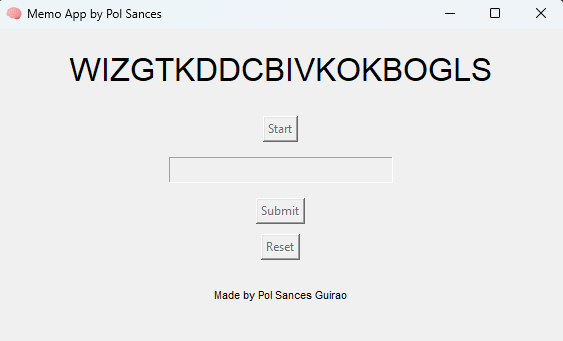
\includegraphics[width=8cm]{img/figures/app-fase2.png}
    \caption{Fase de Memorització}
    \label{fig:fase-memo}
\end{figure}

\begin{figure}[h!]
    \centering
    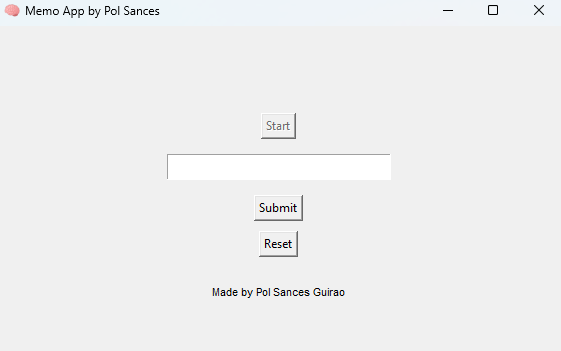
\includegraphics[width=8cm]{img/figures/app-fase3.png}
    \caption{Fase d'introducció de la resposta}
    \label{fig:fase-resp}
\end{figure}
